\documentclass{article}
\title{CSC301 HW4}
\author{Alex Zhang}
\date{Feb 2023}


\textwidth=16.00cm 
\textheight=22.00cm 
\topmargin=0.00cm
\oddsidemargin=0.00cm 
\evensidemargin=0.00cm 
\headheight=0cm 
\headsep=0.5cm
\textheight=610pt

\usepackage{amsthm,amssymb}
\usepackage{amsmath}
\usepackage{graphicx}
\graphicspath{ {./images/} }

\newcommand{\bmat}[1]{\begin{bmatrix} #1 \end{bmatrix}}
\newcommand{\mat}[1]{\mathbf{#1}}
\newcommand{\mb}[1]{\mathbb{#1}}

\let\ds\displaystyle




\begin{document}
\maketitle


\section*{Question 1}
Based on the question, since $n$ is a power of 2, $n$ will always be even. The following is the pesudocode for the algorithm,
\begin{verbatim}
    function v = MEDIAN(A,B,n)
        if n == 1 then return max(A[0],B[0])
        m1 = (A[n/2-1]+A[n/2]) / 2
        m2 = (B[n/2-1]+B[n/2]) / 2
        if m1 == m2 
            then return min(A[n/2],B[n/2])
        if m1 < m2
            return MEDIAN(A[n/2:], B[:n/2], n/2)
        else
            return MEDIAN(A[:n/2], B[n/2:], n/2)
    end function
        
\end{verbatim}
    \subsection*{Proof of Correctness}
    The algorithm assumes that the return value of median will be the number on the right side of two medians.
    In the base case where n = 1, the length of array $A$ and $B$ is 1, which the median of these two arrays are $A[0]$ and $B[0]$. Since the algorithm assumes to
    get the larger median, it will return max number between these two. The base case works.
    \\
    For inductive cases, we assume that the algorithm will work when the length is $n/2$ since $n$ is a power of 2, and we need to show that $n$ length will also work.
    \paragraph*{Case 1:} $m1 = m2$\\
    In this case, in array $A$, there are total $n/2$ numbers that is smaller than $m1$ and there is $n/2$ number bigger than $m1$. This is also same for array $B$ and
    number $m2$. Therefore, in the union of two arrays, there are total $n$ number smaller and $n$ number larger than $m1$, indicating $m1$ or $m2$ is also the median
    of the union of two arrays. Since
    \begin{align}
        m1 &= \frac{(A[n/2-1]+A[n/2])}{2} \nonumber \\
        m2 &= \frac{(B[n/2-1]+B[n/2])}{2} \nonumber        
    \end{align}
    And they are euqal to each other. We can get that larger number between $A[n/2-1]$ and $B[n/2-1]$
    lands at position $n/2 -1$ and the smaller number between $A[n/2]$ and $B[n/2]$ lands as position $n/2$. Based on the algorithm, it will return the larger median which 
    is the the smaller number between $A[n/2]$ and $B[n/2]$.
    
    \paragraph*{Case 2:} $m1 < m2$ \\
    In this case, $m1$ and $m2$ will stil follow the case that in each array, there is going to be $n/2$ smaller and larger than $m1$ and $m2$. However, since $m1 < m2$,
    this means that all number smaller than $m1$ in array $A$ will also be smaller than $m2$. Therefore, there will be more than $n$ number smaller than $m2$ so the true 
    median $m_t$ has the property that
    $$m1 \leq m_t \leq m2$$
    We can then eliminate the left side of $m1$ in array because they are all too small, and also the right side of $m2$ in array $B$ since they are all too big.
    The algorithm does the recursion and then following with computing median based on the new array.
    \paragraph*{Case 3:} $m1 > m2$ \\
    This case is very similar to the case above. Again, in array $A$, there are $n/2$ number smaller than $m1$ and also $n/2$ number bigger than $m1$. This also holds true
    for $m2$. Since $m1 > m2$ this means that the true median will locate between $m1$ and $m2$ Because for the right side of $m1$ in array $A$, the number are too big becuase
    there are at least $n$ number before it. We can also eliminate the left side of $B$ since they are too small. The largest number in left side is smaller than $m2$
    which means only bigger than $n/2 - 2$ numbers. For the algorithm, it chops off the sides where true median will not exist and does the recursion on new arrays.\\
    For second and third cases, each recursion, $n$ is divided by two until $n=1$. Since we assume that $n/2$ is true, the recursion will work. $\blacksquare$

    \subsection*{Costs Analysis}
    For each recursion, the time complexity will be $O(1)$. The addition and division are assumed to be constant time since the number in arrays are not n-bits number. The comparison and splicing
    will also only need constant time and $n$ is a power of 2, $n/2$ costs $O(1)$. Since we assume that the length of two arrays are n-bits numbers, and we are doing the recursion by dividing by two each time until $n=1$.
    $T(1) = O(1)$. We can then thrive the equation,
    $$T(n) = T(n/2) + O(1)$$
    In base case, the comparison also only require constant time, so $T(1) = O(1)$. Assume we have to go through $r$ times of recursive calls until the base case, $r$ can 
    be represented as,
    \begin{align}
        \frac{n}{2^r} &= 1 \nonumber \\
        n &= 2^r  \nonumber \\
        n &= 2^{\log_2 n} \nonumber \\
        r &= \log n \nonumber
    \end{align}
    There are $\log n$ recursions and each recursions cost constant time. We conclude that the running time for this algorithm will be $O(\log n)$.
    
\section*{Question 2}
For this question, we first define that randomly choose a pivot, if the pivot is just in the middle 50 \% of the data, we will call it a good pivot. In each recursion, 
the pivot is chosen to be at worst spliting array into $1/4n$ and $3/4n$ where the array length is $n$. The following is the sample recursion tree:
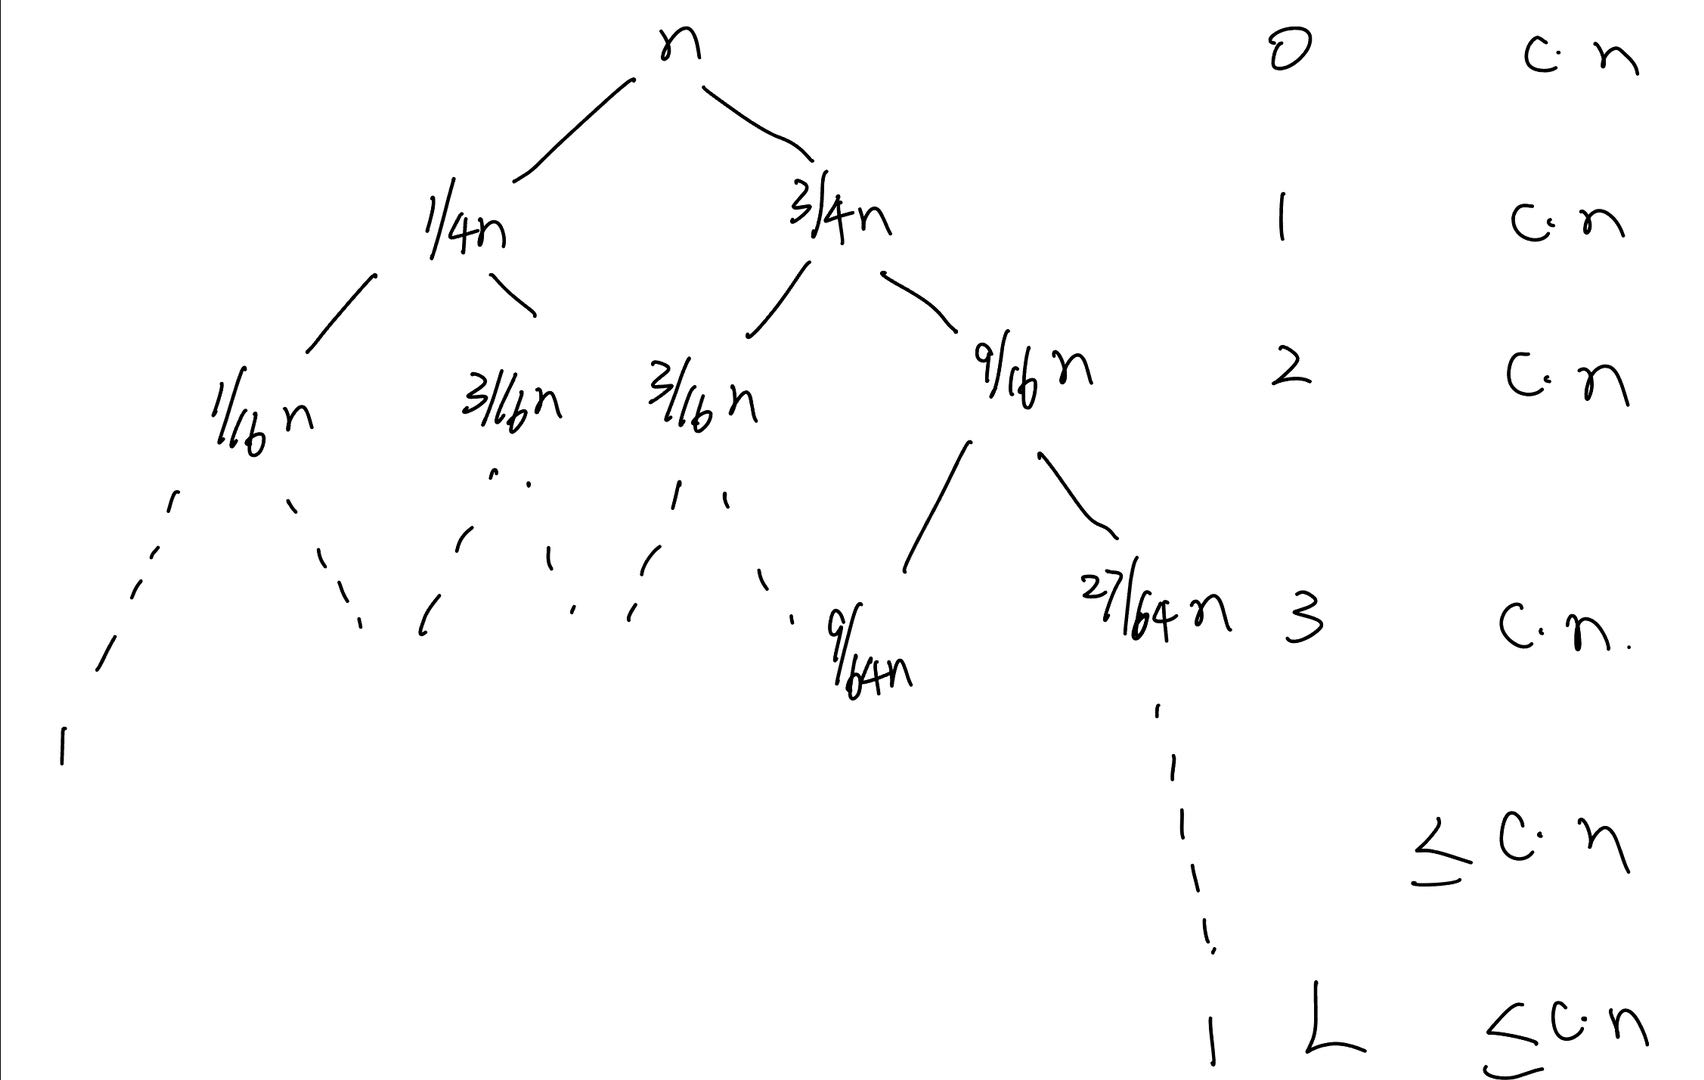
\includegraphics[scale=0.25]{tree2.jpg}\\
In this case, this is not a balanced tree. We assume that in the worst part, the level of tree could
go to $L$ level, which satisfies the equation which 
\begin{align}
    (\frac{3}{4})^L n &= 1 \nonumber \\
    n &= \frac{4}{3}^L \nonumber \\
    n &= \frac{4}{3}^{\log_{\frac{4}{3}}n} \nonumber \\
    L &= \log_{\frac{4}{3}}n \nonumber
\end{align}
So there are total $L+1 = \log_{\frac{4}{3}}n +1$ level. Even though in some branches, base case heppens early, we can still assume that work done in each level
is $cn$. So the total work done has a upper bound
$$\sum_{i=0}^{(\log_\frac{4}{3}n) + 1}  c\cdot n$$
Furthermore, since we are assuming each time pivot will be a good pivot (in the middle 50 \% of data), the expected value of getting into this situation
in each partitioning is $\frac{1}{1/2} = 2$, which means in each recursion, we have to do choose pivot twice to expected pivot lands in this range. So the actual total work is,
$$\sum_{i=0}^{(\log_\frac{4}{3}n) + 1}  c \cdot 2\cdot n$$
which is 
$$ 2\cdot c\cdot n \log_{\frac{4}{3}}n + 2\cdot  c\cdot n$$
Changing the base,
$$2 \cdot c\cdot n \frac{\log_2n}{\log_2\frac{4}{3}} + 2\cdot c\cdot n$$
Since $\log_2\frac{4}{3}$, $2$, and $c$ is a constant, and $2\cdot c\cdot n \frac{\log_2n}{\log_2\frac{4}{3}}$ is the dominating term, we can get the big-Oh for this recursion,
$$O(2 \cdot c\cdot n \frac{\log_2n}{\log_2\frac{4}{3}} + 2\cdot  c\cdot n) = O(n\log_2n)$$
Overall, if we choose a pivot and based on the pivot do the expected runs, we will get the time complexity of $O(n\log_2 n)$. We also showed that the lower bound for quicksort 
is $\Omega(n\log_2 n)$. So the expected running time of quick sort is $\Theta(n\log_2 n)$. $\blacksquare$


\section*{Question 3}
From the lecture, the time complexity for Strassen's algorithm is $O(n^{\log_2 7}) = O(n^{2.81})$. The classical matrix multiplication of partition into $3 \times 3$
grid blocks needs 27 recursive calls and following 18 addtion. We assume that in each recursion, the rest work costs $O(n^2)$ because the input size is $n^2$. We can draw the equation,
\begin{align}
    T(n) &= 27 \cdot T(n/3) + O(18n^2) \nonumber \\
    T(n) &= 27 \cdot T(n/3) + O(n^2) \nonumber
\end{align}
Since $a = 27$, $b = 3$, and $d = 2$, the base case $T(1) = O(1)$, we can use the master theorem. Through master theorem, since $\log_a b > d$, we know that the time complexity will be $O(n^{\log_3 27})$. If we want to create a algorithm which is better than Strassen, we have 
to make sure 
\begin{align}
    O(n^{\log_3 x}) &< O(n^{2.81}) \nonumber \\
    \log_3 x &< 2.81 \nonumber \\
    x &< 3^{2.81} \nonumber\\
    x &< 21.91 \nonumber
\end{align}
Where $x$ is the number of recursive calls. After rounding up, we have to find an algorithm for matrix multiplication with $3\times 3$ parition that only has
$21$ or less recurvie calls in each level to beat Stressen's algorithm. So the largest recursive calls is $21$.




\end{document}